\chapter{Data Analysis}
\label{chapter:data analysis}
\section{Dredging activity}


\section{Hydrodynamic data}
\label{sec 5.2 Hydrodynamic data}
In this section, analysis on the hydrodynamic variables is performed. This includes relations between water elevations, discharge and sediment concentrations - both through data sources and field measurements. Additionally, tidal effects in the study area are considered. 

\subsection{Conversion to water elevation}
A uniform approach is needed to describe water levels and depths of the river. Therefore, these variables will be expressed in terms of a reference level, IGN, which is set by the \textit{Instituto Geográfico Nacional}. It is based on sea level measurements from a tide gauge in Mar del Plata, Buenos Aires province. Figure \ref{fig:waterelevationreference} gives an overview of the quantities with respect to an arbitrary measurement station. Here, \textit{d} is the depth as measured by the ADCP or echosounder. 

\begin{figure}
    \centering
    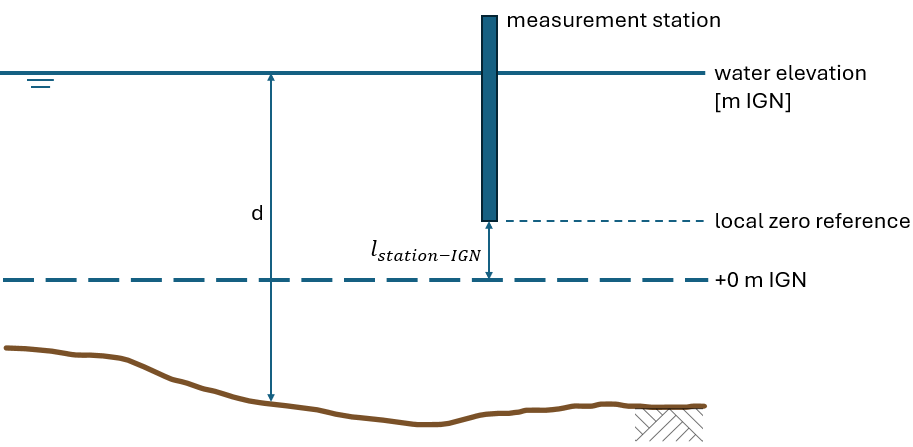
\includegraphics[width=0.75\linewidth]{figures/ch5/waterelevations.png}
    \caption{Water elevation reference}
    \label{fig:waterelevationreference}
\end{figure}






\subsection{Tidal forcing}
The tidal wave of the Atlantic Ocean influences the hydrodynamics of the lower Paraná delta. As the tidal wave enters the delta ta Río de la Plata, the tide is damped and phased by friction, channel geometry and branching, resulting in a reduced amplitude and an increased in phase delay. Under normal conditions, the influence of the tide on the Paraná River reaches the city of Villa Constitución, which is located 220 km upstream of the river mouth. For storm conditions, the tide can reach the city of Rosario \autocite{balayCAUSESPERIODICITYLARGE1958}. In order to determine the influence of the tide at Brazo Largo, a reference water level at San Fernando is considered. It is assumed that at San Fernando no tidal damping has occurred, therefore the tidal amplitude at Brazo Largo can be determined using the following relation:

\begin{equation}
    A_{\text{Location}} = \alpha \cdot A_{\text{SanFernando}}
\end{equation}

The damping coefficient ($\alpha$) and the tidal delay with respect to San Fernando have been determined by Brok (2022). For Brazo Largo, a damping coefficient of 0.3 and tidal delay of 4 hours were found. These values will be used as reference values when isolating the tide at Brazo Largo. The tidal signal is isolated using hourly water level data for a period of more than 2 years from both Brazo Largo and San Fernando. Table 5.2 shows the tidal constituents  considered and their period.

\begin{table}[h!]
\centering
\caption{Tidal constituents used to reconstruct the tide
\autocite{BRON}.}
\label{tab:constituents}
\begin{tabular}{lccc}
\hline
\textbf{Tidal constituent} & \textbf{Name} & \textbf{Period [h]} \\
\hline
\multicolumn{3}{l}{\textit{Semi-diurnal}} \\
\hspace{1em}Principal lunar & M2 & 12.4206\\
\hspace{1em}Principal solar & S2 & 12.0000 \\
\hspace{1em}Lunar elliptical & N2 & 12.6583\\
\hline
\multicolumn{3}{l}{\textit{Diurnal}} \\
\hspace{1em}Lunar-solar declinational & K1 & 23.9345  \\
\hspace{1em}Principal lunar & O1 & 25.8193  \\
\hline
\multicolumn{3}{l}{\textit{Shallow water constituents}} \\
\hspace{1em}Overtide of M2 (quarter-diurnal) & M4 & 6.2103  \\
\hline
\end{tabular}
\end{table}

- uitleg hoe het getijde bepaald is

The tidal amplitude and phase of each constituent for San Fernando and Brazo Largo are displayed in Table 5.3. Additionally, the damping coefficient ($\alpha$) and the tide delay are calculated for the different constituents and shown in Table 5.3. The calculated amplitudes show that the delta has mixed tidal dynamics  (semidiurnal-diurnal)
dominated by the semi-diurnal M2 constituent with contributions from N2, K1 and O1. The overtide M4 plays a minor role. The damping coefficient is consistent across the constituents ranging from 0.23 to 0.33, inditcating that the use of formula 5.3 is valid. The calculated time delay of 4.5 - 5.5 hours is also in line with the time delay calculated by Brok (2022). The damping coefficient of M4 is different because it is generated locally with nonlinear interactions.

\begin{table}[h!]
\centering
\caption{Amplitude and phase comparison}
\begin{tabular}{lcccccc}
\hline
Constituent & $A_{\text{SF}}$ & $A_{\text{BL}}$ & $\alpha$ & tide delay [hr] & $\phi_{\text{SF}}$ [$^\circ$] & $\phi_{\text{BL}}$ [$^\circ$] \\
\hline
M2 & 0.253 & 0.058 & 0.230 & 4.450 & -0.465 & 1.786 \\
S2 & 0.041 & 0.010 & 0.239 & 5.055 & -2.526 & 0.121 \\
N2 & 0.094 & 0.022 & 0.238 & 4.316 & -0.546 & 1.596 \\
K1 & 0.119 & 0.037 & 0.313 & 5.181 & -2.543 & -1.183 \\
O1 & 0.187 & 0.061 & 0.328 & 5.517 & 2.694 & -2.247 \\
M4 & 0.030 & 0.006 & 0.189 & -1.495 & -2.608 & 2.162 \\
\hline
\end{tabular}
\end{table}

Figure 5.7 shows the water level time series for a period of 7 days compared to the calculated tidal signal at Brazo Largo. From this figure, it can be seen that the measured water level follows the same tidal oscillations. However, the tide does not explain all the variability of the water level; the measured water level also shows large variability caused by discharge and wind. 
\\The influence of the strong non-tidal component is confirmed by Figure 5.8, which shows the water level at Brazo Largo for a period of 2 years. The measured water level fluctuates greatly, reaching +2.0 m and -0.5 m while the tidal component is steady at 0.0 m with an amplitude of 0.17 m. The tidal forcing is relatively small compared to the river and seasonal influences. Tidal forcing is therefore subordinate to other forcings such as discharge.

\begin{figure}[H]
    \centering
    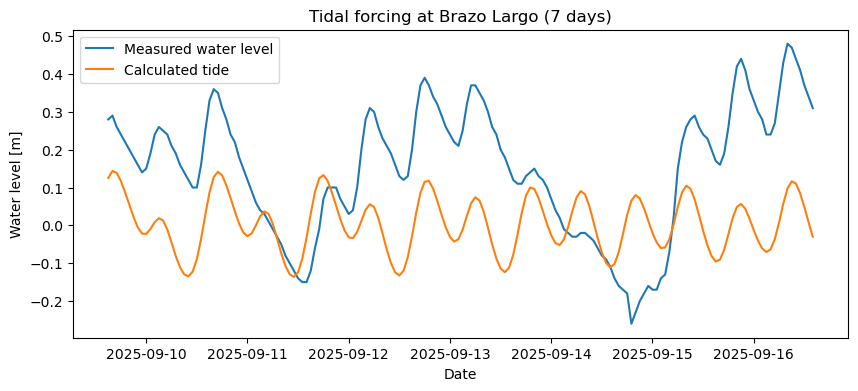
\includegraphics[width=1\linewidth]{figures/ch5/Tide_Brazo_largo.png}
    \caption{Calculated tide at Brazo Largo for a period of 7 days.}
    \label{fig:placeholder}
\end{figure}
\begin{figure}[H]
    \centering
    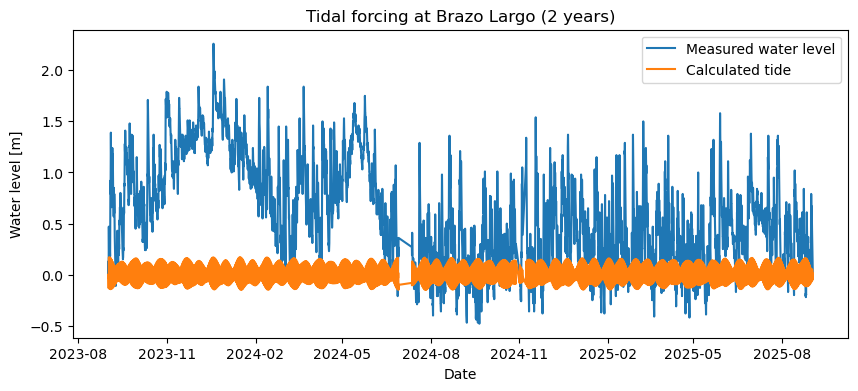
\includegraphics[width=1\linewidth]{figures/ch5/Tide_BL_2y.png}
    \caption{Calculated tide at Brazo Largo for a period of 2 years.}
    \label{fig:placeholder}
\end{figure}

- Waterlevel at Brazo Largo
    (misschien het getijde meenemen?)
\\ - Getijde rond Brazo Largo is berekend aan de hand van waterlevel rond San Fernando. Vergelijk de constituents met die van  het rapport en trek conclusie over invloed getijde.

\subsection{Fluvial forcing}

The relationship between fluvial discharge and water level at Brazo Largo was initially assumed to follow a power-law ($h = a \cdot Q^b$), but this yielded a weak correlation with an $R^2$ of 0.261. A linear fit, however, produced a slightly better result, showing a positive trend with an $R^2$ of 0.444 (Figure \ref{fig:waterleveldischarge}).

In contrast, the El Colorado and Túnel Subfluvial stations exhibit a clear power-law dependence. Power-law fits for these stations resulted in higher $R^2$-values of 0.962 and 0.712, respectively, with the El Colorado plot shown in Figure \ref{fig:waterleveldischarge}. Overall, these results suggest that the strength of the water level–discharge relationship decreases as the river flows downstream.

\begin{figure}[h!]
    \centering
    % First subfigure
    \begin{subfigure}[b]{0.48\linewidth}
        \centering
        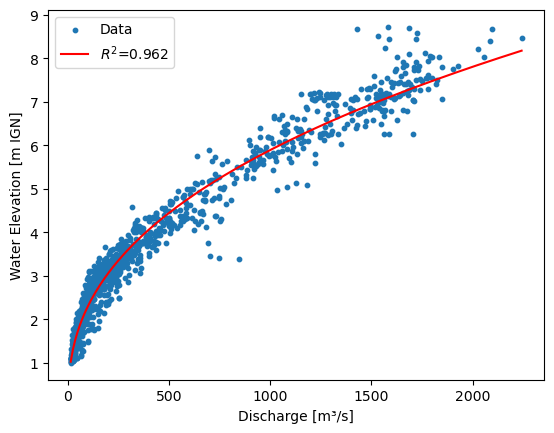
\includegraphics[width=\linewidth]{figures/ch5/wl discharge El Colorado.png}
        \label{fig:water level discharge Colorado}
    \end{subfigure}
    \hfill
    % Second subfigure
    \begin{subfigure}[b]{0.48\linewidth}
        \centering
        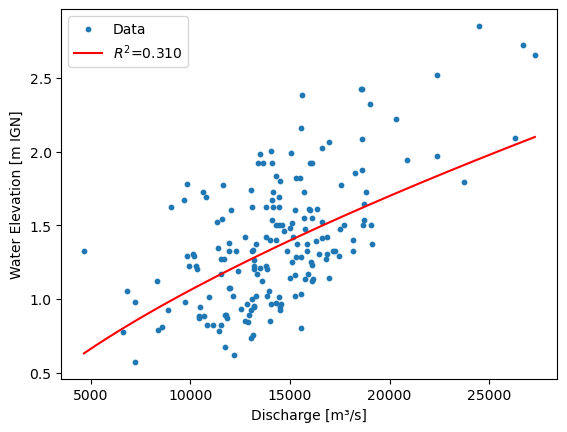
\includegraphics[width=\linewidth]{figures/ch5/wl discharge Brazo Largo.png}
        \label{fig:water level discharge Brazo Largo}
    \end{subfigure}
    \caption{Water elevation - discharge relationship for two measurement stations}
    \label{fig:waterleveldischarge}
\end{figure}



\subsection{Flow partitioning}

At some point in the Lower Paraná, the river splits into two main tributaries, as shown in Figure \ref{fig:flow partition}. To have an approximation for the distribution of discharge between these rivers, the discharge series are given in Figure \ref{fig:discharge_series}. From these plots, it follows that the majority of the discharge flows into the Paraná Guazú. Figure \ref{fig:flow_partition} represents this ratio and plots a linear fit. As there is no significant increase or decrease, the approximation is made that 78\% of the total discharge upstream of the confluence flows into Paraná Guazú. \citeauthor{reMETODOLOGIAPARAGENERACION2009} report that a linearly increasing trend occurs. Here, more data is used and therefore the approximation of a constant percentage is applied. 

In order to further study the liquid flows in the Paraná Guazú, it is noted that estimates for the discharge of Río Ibicuy and Río Talabera are needed. These were collected during the fieldwork, as indicated in Figure \ref{fig:fieldwork cross sections}.

\begin{figure}[h!]
    \centering
    % First subfigure
    \begin{subfigure}[b]{0.48\linewidth}
        \centering
        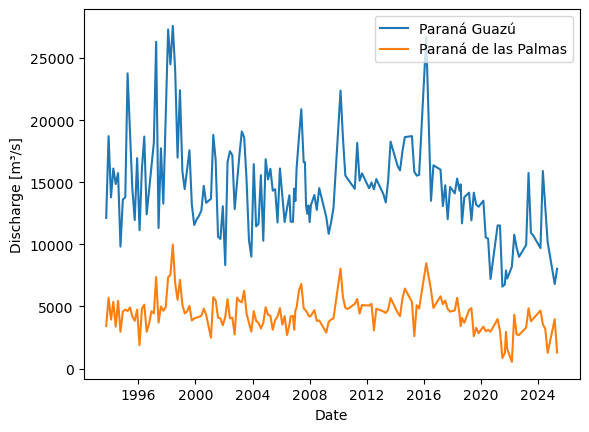
\includegraphics[width=\linewidth]{figures/ch5/discharge series.png}
        \caption{Discharge series obtained from Brazo Largo and Zárate measurement stations}
        \label{fig:discharge_series}
    \end{subfigure}
    \hfill
    % Second subfigure
    \begin{subfigure}[b]{0.48\linewidth}
        \centering
        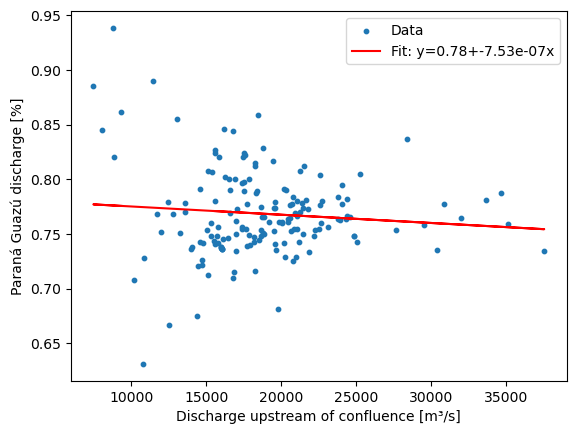
\includegraphics[width=\linewidth]{figures/ch5/flow partition.png}
        \caption{Flow partition, expressed as the share of total flow that streams into Paraná Guazú}
        \label{fig:flow_partition}
    \end{subfigure}
    
    \caption{Comparison between (a) discharge series and (b) flow partition of the Paraná Guazú and Paraná de las Palmas}
\end{figure}



\section{Sediment transport}
From the Brazo Largo measurements, an analysis can be done on the relationship between sediment concentrations and the discharge of the river. Again, a distinction can be made between fine and course sediments. Overall, a power-law fit seems a good approach to model the relation, as shown in Figure \ref{fig:sediments discharge}. The fine sediment concentration is generally higher than the course sediment concentration. In addition, the course sediment concentration increases more significantly for an increasing fluvial discharge. These are general trends, but it has to be stressed that the $R^2$ of both relationships is relatively low. 

\begin{figure}
    \centering
    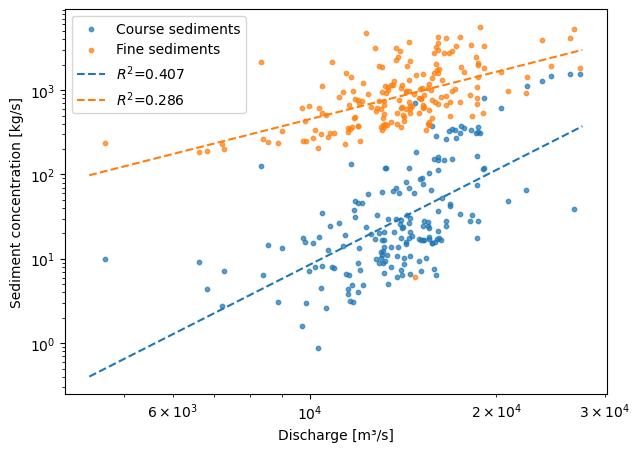
\includegraphics[width=0.5\linewidth]{figures/ch5/Discharge sediment relation.png}
    \caption{Fine and course sediment concentrations in relation to discharge at Brazo Largo}
    \label{fig:sediments discharge}
\end{figure}



- Bepaal fine sediment-discharge relation bij El Colorado. Reken hiermee door voor het fine sediment concentration bij Brazo Largo

- Bepaal fine sediment concentration op basis van de suspended sediment samples.

- Coarse sediment concentration wordt bepaald met de Engelund-Hansen formule

- Vergelijk dit met de bedload metingen van het veldwerk

- Set up a sediment balance for the area of interest.


- Sediment transport caused by tidal assymetry.
% \section{Water Quality and Bioorganism Activity?}

